\section{Tarski and Russell universes (\ThyTarski and \ThyRussell)}\label{sectionT1T2}

We now prove the main result of the paper : equivalence of Tarski-style and Russell-style universes i.e. of \ThyTarski and \ThyRussell.
All the results of this section have been completely formalised \textit{by hand} in Rocq.

First, we show that the erasure operation $|.|$ preserves derivations.

\begin{lemma}[\formline{Erasure.v}{143}{Erasurecorrection} Correctness of erasure]
    If $\Gamma \vdash J$ in \ThyTarski, then $|\Gamma| \vdash |J|$ in \ThyRussell.
\end{lemma}

\begin{proof}
    By mutual induction, we prove the statement for our five different kinds of judgements: well-formation of contexts and types,
    typing, and conversion between types and terms. The proof is mostly direct, and amounts to showing that the
    erasure of each rule of \ThyTarski corresponds to an admissible rule of \ThyRussell.
\end{proof}

Then, we want to show that this forgetful map has an inverse, hence proving the equivalence
of the two systems. For this, we will need some technical lemmas, which we all prove simultaneously by a mutual
induction on the derivation.

\begin{lemma}[\formline{Utils.v}{330}{Hypothesis} Hypothesis inversion]\label{hyp-inv}
    If we have a derivation $\Gamma, A \vdash J$, where $J$ is an arbitrary judgment,
    then we necessarily have a derivation $\Gamma \vdash A \; \type$.
\end{lemma}

\begin{lemma}[\formline{Utils.v}{1050}{Hypothesis} Typing and conversion inversion]

    If we have a derivation $\Gamma \vdash a : A$ or $\Gamma \vdash a = b :A$ then we necessarily have a derivation $\Gamma \vdash A \; \type$.
\end{lemma}

Those two lemmas allow us to reason by inversion on given judgements, as Rocq's inversion
tactic would be stuck with rules such as :
\begin{mathparsmall}
  \ebrule{
    \hypo{\Gamma \vdash a : A}
    \hypo{\Gamma \vdash A = B}
    \infer2{\Gamma \vdash a : B}
  }
\end{mathparsmall}

We also need the following lemma, which will allow us to modify derivations given a conversion judgement.

\begin{lemma}[\formline{Utils.v}{1059}{Hypothesis}]\label{Transform}
    If we have a derivation $\Gamma, A \vdash J$ and a convertibility derivation $\Gamma \vdash A = B$,
    then we can construct a derivation $\Gamma, B \vdash J$.
\end{lemma}

Now, we would want to state the main result, by adapting the arguments of \citet{Streicher}. One could try to prove the
following statement:\\

\textbf{Lemma.} If we have $\Gamma \vdash u_0 : A_0$ and $\Gamma \vdash u_1 : A_1$ such that $|u_0| = |u_1|$
in \ThyRussell, then necessarily they are convertible i.e. $\Gamma \vdash A_0 = A_1$ and $\Gamma \vdash u_0 = u_1 : A_0$\\

However, this fails when $u_0$ and $u_1$ are codes in different universes. For instance, we have $\Gamma \vdash \U_m^n : \U_n$ and $\Gamma \vdash \U_m^l : \U_l$
which have the same erasure $|\U_m^n| = |\U_m^l| = \U_m$, but are not convertible (at least if $n \neq l$). Therefore,
we need to prove a more general statement that properly deals with the case when $A_0$ and $A_1$ are universes. In this case, we should 
be able to find a lower universe, and two convertible terms in that lower universe, which lift to $u_0$ and $u_1$ respectively. This correspond to the 
following figure:

\begin{figure}[H]
\centering
\resizebox{0.42\textwidth}{!}{%
    
    

\tikzset{every picture/.style={line width=0.75pt}} %set default line width to 0.75pt        

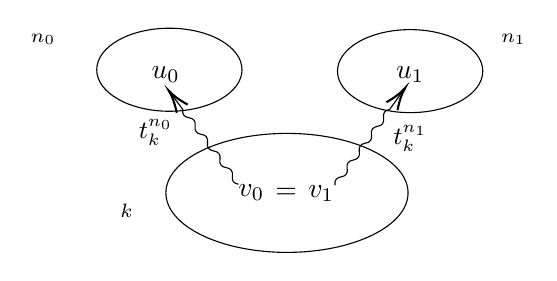
\begin{tikzpicture}[x=0.75pt,y=0.75pt,yscale=-1,xscale=1]
%uncomment if require: \path (0,300); %set diagram left start at 0, and has height of 300

%Shape: Ellipse [id:dp4815941303797192] 
\draw   (103.67,84.33) .. controls (103.67,73.29) and (119.34,64.33) .. (138.67,64.33) .. controls (158,64.33) and (173.67,73.29) .. (173.67,84.33) .. controls (173.67,95.38) and (158,104.33) .. (138.67,104.33) .. controls (119.34,104.33) and (103.67,95.38) .. (103.67,84.33) -- cycle ;
%Shape: Ellipse [id:dp17791572333330286] 
\draw   (219.67,85) .. controls (219.67,73.95) and (235.34,65) .. (254.67,65) .. controls (274,65) and (289.67,73.95) .. (289.67,85) .. controls (289.67,96.05) and (274,105) .. (254.67,105) .. controls (235.34,105) and (219.67,96.05) .. (219.67,85) -- cycle ;
%Shape: Ellipse [id:dp467313711776734] 
\draw   (137,143.67) .. controls (137,127.83) and (163.12,115) .. (195.33,115) .. controls (227.55,115) and (253.67,127.83) .. (253.67,143.67) .. controls (253.67,159.5) and (227.55,172.33) .. (195.33,172.33) .. controls (163.12,172.33) and (137,159.5) .. (137,143.67) -- cycle ;
%Straight Lines [id:da3638554959651593] 
\draw    (172,139.5) .. controls (169.67,139.16) and (168.67,137.82) .. (169.01,135.49) .. controls (169.35,133.16) and (168.35,131.82) .. (166.02,131.48) .. controls (163.69,131.14) and (162.69,129.8) .. (163.04,127.47) .. controls (163.38,125.14) and (162.38,123.8) .. (160.05,123.46) .. controls (157.72,123.13) and (156.72,121.79) .. (157.06,119.46) .. controls (157.4,117.13) and (156.4,115.79) .. (154.07,115.45) .. controls (151.74,115.11) and (150.74,113.77) .. (151.08,111.44) .. controls (151.42,109.11) and (150.42,107.77) .. (148.09,107.43) .. controls (145.76,107.09) and (144.76,105.75) .. (145.11,103.42) -- (144.31,102.35) -- (139.53,95.94) ;
\draw [shift={(138.33,94.33)}, rotate = 53.3] [color={rgb, 255:red, 0; green, 0; blue, 0 }  ][line width=0.75]    (10.93,-3.29) .. controls (6.95,-1.4) and (3.31,-0.3) .. (0,0) .. controls (3.31,0.3) and (6.95,1.4) .. (10.93,3.29)   ;
%Straight Lines [id:da2882231844046552] 
\draw    (218.5,140) .. controls (218.12,137.67) and (219.09,136.32) .. (221.42,135.94) .. controls (223.75,135.56) and (224.72,134.21) .. (224.34,131.88) .. controls (223.96,129.55) and (224.93,128.2) .. (227.26,127.83) .. controls (229.59,127.45) and (230.56,126.1) .. (230.18,123.77) .. controls (229.81,121.44) and (230.78,120.09) .. (233.11,119.71) .. controls (235.44,119.33) and (236.41,117.98) .. (236.03,115.65) .. controls (235.65,113.32) and (236.62,111.97) .. (238.95,111.59) .. controls (241.28,111.22) and (242.25,109.87) .. (241.87,107.54) .. controls (241.49,105.21) and (242.46,103.86) .. (244.79,103.48) -- (246.49,101.12) -- (251.16,94.62) ;
\draw [shift={(252.33,93)}, rotate = 125.75] [color={rgb, 255:red, 0; green, 0; blue, 0 }  ][line width=0.75]    (10.93,-3.29) .. controls (6.95,-1.4) and (3.31,-0.3) .. (0,0) .. controls (3.31,0.3) and (6.95,1.4) .. (10.93,3.29)   ;

% Text Node
\draw (128.83,81.4) node [anchor=north west][inner sep=0.75pt]  [font=\normalsize]  {$u_{0}$};
% Text Node
\draw (70.67,65.73) node [anchor=north west][inner sep=0.75pt]  [font=\normalsize]  {$\U_{n_{0}}$};
% Text Node
\draw (246.67,81.57) node [anchor=north west][inner sep=0.75pt]  [font=\normalsize]  {$u_{1}$};
% Text Node
\draw (297.33,65.73) node [anchor=north west][inner sep=0.75pt]  [font=\normalsize]  {$\U_{n_{1}}$};
% Text Node
\draw (170.67,138.23) node [anchor=north west][inner sep=0.75pt]  [font=\normalsize]  {$v_{0}$};
% Text Node
\draw (204.33,138.73) node [anchor=north west][inner sep=0.75pt]  [font=\normalsize]  {$v_{1}$};
% Text Node
\draw (113.83,147.73) node [anchor=north west][inner sep=0.75pt]  [font=\normalsize]  {$\U_{k}$};
% Text Node
\draw (122.67,107.07) node [anchor=north west][inner sep=0.75pt]  [font=\small]  {$t_{k}^{n_{0}}$};
% Text Node
\draw (245.33,109.73) node [anchor=north west][inner sep=0.75pt]  [font=\small]  {$t_{k}^{n_{1}}$};
% Text Node
\draw (188.5,140.4) node [anchor=north west][inner sep=0.75pt]  [font=\normalsize]  {$=$};


\end{tikzpicture}


}%

\label{fig:my_label}
\end{figure}

Even with this generalised lemma, we would get stuck in the proof for the case of the decoding. Indeed, if we have a code $a: \U_n$ and a type $A$ 
whose erasure is $|A| = |a|$, then we cannot deduce much on $A$ itself as it could well be any type.
Nevertheless, we still know that $\Gamma \vdash A : \U_n$ holds in Russell-style because it is the same syntactic term as $a$. This should indicate that $A$ is a small type, i.e. a decoded type, and
in this setting we will prove that : \[\Gamma \vdash A = T_n(a)\]

Thus, we shall prove the following lemma, which is one of the most technical result of this paper. 

\begin{lemma}[\formline{Equivalence.v}{813}{eraseinjty}] \label{mainuniverse}
    In \ThyTarski, we have:
    \begin{enumerate}
    \item If $\Gamma \vdash A\; \type$ and $\Gamma \vdash B\; \type$ with $|A| = |B|$, then  $\Gamma \vdash A = B$.

    \item If $\Gamma \vdash t : \U_n$ and $\Gamma \vdash A \; \type$ with $|A| = |t|$, then $\Gamma \vdash A = T_n(t)$. 

    \item If $\Gamma \vdash u_0 : A_0$ and $\Gamma \vdash u_1 : A_1$ with $|u_0| = |u_1|$, then we have two cases:
    \begin{itemize}
        \item Either $\Gamma \vdash A_0 = A_1$ and $\Gamma \vdash u_0 = u_1 : A_0$.
        \item Or they are codes, such that $\Gamma \vdash A_0 = \U_{n_0}$, $\Gamma \vdash A_1 = \U_{n_1}$, and 
            there exists two convertible terms $\Gamma \vdash v_0 = v_1 : \U_k$ in a lower universe, which
            lifts to $u_0$ and $u_1$:

            \vspace{0.5em}

            \noindent
            \begin{minipage}{0.5\linewidth}
                \centering
                $\Gamma \vdash u_0 = t_k^{n_0}(v_0) : A_0$
            \end{minipage}
            \hfill
            \begin{minipage}{0.5\linewidth}
                \centering
                $\Gamma \vdash u_1 = t_k^{n_1}(v_1) : A_1$
        \end{minipage}
    \end{itemize}
    \end{enumerate}
\end{lemma}

\begin{proof}
    We prove the property by mutual induction on $A$ and $u_0$, proving the three statements at the same time. For each of the cases of
    the induction, we need a "catch-up" lemma which inverts the erasure hypothesis. Concretely the issue is that we cannot 
    deduce from $|u_1| = \Pi(A,B)$ that $u_1$ is a dependent product, as it could well be the decoding of a code $T_n(\Pi^n \; a \; b)$, or
    even a decoding of a lift $T_n(t_m^n(a))$. To solve this, we need to do another induction on $u_1$ for each case.

    We now present some of the key cases of the proof.\\

    \textit{Lambda abstraction.} If $u_0 = \lambda(C_0,B_0,b_0)$, then we necessarily have $\Gamma \vdash A_0 = \Pi(C_0,B_0)$,
        and by inversion, the derivation $\Gamma \vdash u_0 : A_0$ looks like :

    \begin{mathparsmall}
      \ebrule{
        \hypo{\Gamma.C_0 \vdash b_0 : B_0}
        \infer1{\Gamma \vdash \lambda(C_0,B_0,b_0) : \Pi(C_0,B_0)}
      }
    \end{mathparsmall}

    Then $|u_0| = \lambda(|C_0|, |B_0|, |b_0|) = |u_1|$ and so $u_1$ is necessarily
    an abstraction or a lift. Now let's prove the property by induction on $u_1$.

    \begin{itemize}
        \item \underline{First case:} $u_1 = \lambda(C_1, B_1, b_1)$ with $|C_1| = |C_0|$, $|B_1| = |B_0|$, $|b_1| = |b_0|$.
    Also, by inversion $\Gamma \vdash u_1 : A_1$ is necessarily of the same shape. 
    Using the induction hypothesis on $C_0$ with $C_1$, we get $\Gamma \vdash C_0 = C_1$.
    Then, by lemma \ref{Transform} we get a derivation
    $\Gamma,C_0 \vdash b_1 : B_1$. Now we can apply the induction hypothesis on $b_0$ with $b_1$, and get two cases. 
    
    In the first case, we get directly derivations $\Gamma.C_0 \vdash b_1 = b_0 : B_0$ and $\Gamma.C_0 \vdash B_0 = B_1$,
    and using congruence equations we obtain the desired $\Gamma \vdash u_0 = u_1 : A_0$.
    
    In the second case, we get $\Gamma \vdash A_0 = \U_{n_0}$, from which we deduce $\Gamma \vdash \Pi(C_0,B_0) = \U_{n_0}$,
    which is a contradiction by Theorem \ref{no-confusion}.

    \item \underline{Second case:} $u_1 = t_n^m(a)$, and we will show that this case is not possible.
        Indeed, we thus have $A_1 = \U_m$ and $|u_1| = |a| = |u_0|$ and we can apply the induction hypothesis
        on $a$, and in each case we obtain either $\Gamma \vdash A_0 = \U_m$ or $\Gamma \vdash A_0 = \U_{n_0}$, which
        are absurd because of lemma \ref{no-confusion}.
    \end{itemize}

    The case of lambda abstraction illustrated the main arguments used, and how no-confusion plays an 
    essential role to our arguments. However, in more complicated cases, we cannot always eliminate lifting
    cases.\\

    \textit{Code for a universe.} If $u_0$ is a code for a universe, then by inversion :
    \begin{mathparsmall}
      \ebrule{
        \hypo{}
        \infer1{\Gamma \vdash \U_m^{n_0} : \U_{n_0}}
      }
    \end{mathparsmall}
    Then $|u_0| = \U_m = |u_1|$ so we have two cases either $u_1 = \U_m^{n_1}$ or $u_1 = t_l^{n_1} (\U_m^l)$.

    \begin{itemize}
        \item \underline{First case :} We have $u_1 = \U_m^{n_1}$, and by inversion
    the following derivations : $\Gamma \vdash A_0 = \U_{n_0}$ and $\Gamma \vdash A_1 = \U_{n_1}$.
    If we define $k := \min{n_0,n_1}$ then we can construct derivations
    $\Gamma \vdash u_0 = t_k^{n_0} (\U_m^k)$ and $\Gamma \vdash u_1 = t_k^{n_1} (\U_m^k)$, with $\Gamma \vdash \U_m^k = \U_m^k : \U_k$.

    \item \underline{Second case :} We have $u_1 = t_l^{n_1} (\U_m^l)$, and by inversion the following
    derivations : $\Gamma \vdash A_0 = \U_{n_0}$ and $\Gamma \vdash A_1 = \U_{n_1}$. If we define $k := \min(l,n_0)$, we can construct derivations
    $\Gamma \vdash u_0 = t_k^{n_0} (\U_m^k)$ and $\Gamma \vdash u_1 = t_k^{n_1} (\U_m^k)$, with  $\Gamma \vdash \U_m^k = \U_m^k : \U_k$.
    \end{itemize}
\end{proof}



\begin{lemma}[\formline{Equivalence.v}{11}{simplifyinduction}]\label{Utile}
     Let's assume that : $\Gamma \vdash A_0 = \U_{n_0}$, $\Gamma \vdash A_1 = \U_{n_1}$ and 
     $\Gamma \vdash u_0 = t_k^{n_0}(v_0) : A_0$, $\Gamma \vdash u_1 = t_k^{n_1}(v_1) : A_1$ with
     $\Gamma \vdash v_0 = v_1 : \U_k$.

     Then if we additionally have  $\Gamma \vdash A_0 = A_1$, we get : $\Gamma \vdash u_0 = u_1: A_0$.
\end{lemma}
\begin{proof}
    By transitivity, we get $\Gamma \vdash \U_{n_0} = \U_{n_1}$ from which we can deduce $n_0 = n_1$ using
    injectivity of universes. Hence, $u_0$ and $u_1$ are codes living in the same universe.
    Via congruence, we get $\Gamma \vdash t_k^{n_0}(v_0) = t_k^{n_0}(v_1)$,
    from which we deduce $\Gamma \vdash u_0 = u_1 : A_0$ by transitivity.
\end{proof}


Hence, we deduce the following corollary, which states that if we have two judgments
in \ThyTarski which are syntactically equal in \ThyRussell (when removing coercions, lifts...), then
they are provably convertible in \ThyTarski. This already means that the Tarski system is not much stronger than
the Russell one, in the sense that if two terms differ only by their explicit coercion, then they have the same
computational behaviour.

\begin{corollary}[\formline{Equivalence.v}{1128}{eraseinjtermplus} Judgemental injectivity of erasure]\label{uniqueness}
    If $\Gamma \vdash u_0 : A_0$ and $\Gamma \vdash u_1 : A_1$ in \ThyTarski and $|u_0| = |u_1|$,
    with the additional hypothesis $|A_0| = |A_1|$, then : $\Gamma \vdash A_0 = A_1$ and 
    $\Gamma \vdash u_0 = u_1 : A_0$.
\end{corollary}

\begin{proof}
    We apply lemma \ref{mainuniverse} on the equality $|A_0| = |A_1|$ to get $\Gamma \vdash A_0 = A_1$, and on
    $|u_0| = |u_1|$ to get the two cases. In the first one, we directly have $\Gamma \vdash u_0 = u_1 : A_0$,
    and in the second one, we use lemma \ref{Utile} to get the derivation.
\end{proof}

Now we prove the following theorem, stating the formal equivalence between the two systems:

\begin{theorem}[\formline{Equivalence.v}{1379}{sectionctx} Section of erasure]\label{equT1T2}
    If $\Gamma \vdash J$ in the system \ThyRussell, then there exists a unique, up to conversion judgment
    $\Gamma_1 \vdash J_1$ in the system \ThyTarski such that $|\Gamma_1| = \Gamma$ and $|J_1| = J$.
\end{theorem}

\begin{proof}
    Uniqueness up to conversion follows directly from the previous lemma. We have to construct the derivation 
    by induction on the rules of \ThyRussell, making an extensive use of the previous lemma for rules with two premises. Indeed,
    when using the induction hypothesis on two premises, we need to make sure that the same types have 
    the same translations. To illustrate this, we detail the case of the product.\\

    \textit{Dependent Product.} If the last rule applied in \ThyRussell is :
    \begin{mathparsmall}
      \ebrule{
        \hypo{\Pi_1}
        \infer1{\Gamma \vdash A \; \type}
        \hypo{\Pi_2}
        \infer1{\Gamma.A \vdash B \; \type}
        \infer2{\Gamma \vdash \Pi(A,B) \; \type}
      }
    \end{mathparsmall}

        Then, by the induction hypothesis we get derivations 
        $\Gamma' \vdash A' \; \type$ and $\Gamma'',A'' \vdash B' \; \type$ in \ThyTarski such that 
         $|\Gamma'| = |\Gamma''| = \Gamma$ and $|A''| = |A'| = A$. By Corollary \ref{uniqueness}, we get $\Gamma' \vdash A' = A''$, and  the contexts
        $\Gamma'$ and $\Gamma''$ are convertible. We can thus transform the second derivation to get $\Gamma',A' \vdash B' \; \type$.
        Therefore, we can construct the derivation for $\Gamma' \vdash \Pi(A',B') \; \type$ in \ThyTarski.
\end{proof}

This finally proves that any judgement in Russell-Style can be lifted uniquely to a judgement in Tarski-Style, proving
the equivalence between \ThyTarski and \ThyRussell by exhibiting a section of the forgetful map.

\begin{remark}
To prove this equivalence result, we could have relied on normalisation to simplify the proofs, at
the cost of relying on a stronger metatheory and stronger properties of the theory. In fact, if we proved normalisation for
\ThyRussell as well, we could construct the derivation of Theorem \ref{equT1T2} by an induction on normal forms.
Then, by showing that the erasure map $|.|$ commutes with $\nf(.)$, we would obtain the equivalence result.
\end{remark}
